\chapter{Obiekt regulacji}
\label{cha:ch2_obiekt_regulacji}

Obiektem poddawanym regulacji był system typu kulka na belce, który został zbudowany od podstaw na potrzeby tej pracy.

\section{Obiekty typu kulka na belce}

Na system tego typu składają się długa, umieszczona horyzontalnie belka i silnik lub serwomechanizm, który umożliwia wychylanie się belki.
Po belce swobodnie porusza się kulka.

Podstawowym zadaniem regulacji w systemie tego typu jest stabilizacja położenia kulki w wybranym punkcie.
Charakterystyczną cechą tego systemu jest prostota konstrukcji oraz niestabilność przy braku aktywnej regulacji.

Obiekty tego typu są często wykorzystywane w dydaktyce teorii sterowania. Składają się na to poniższe powody:

\begin{itemize}
	\item prostota budowy,
	\item możliwość zastosowania różnych czujników położenia kulki,
	\item możliwość zastosowania różnych silników i mechanizmów przeniesienia napędu.
\end{itemize}

Uproszczony schemat systemu kulka i belka przedstawiony został poniżej:

\begin{figure}[H]
	\centering
	\includesvg[width=0.7\textwidth]{kulka_belka_schemat_uproszczony}
	\caption{Uproszczony schemat systemu typu kulka i belka.}
	\label{fig:kulka_belka_schemat_uproszczony}
\end{figure}

Stąd też dostępne są komercyjne obiekty przygotowane dla laboratoriów sterowania cyfrowego, jak na przykład produkt firmy Quanser.

\begin{figure}[H]
	\centering
	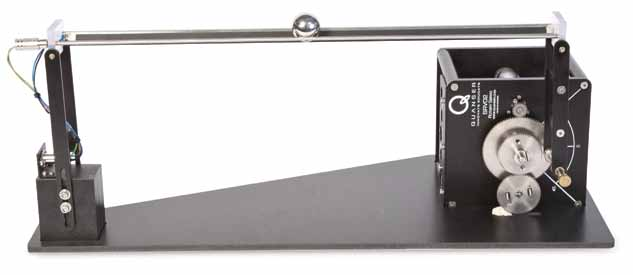
\includegraphics[width=0.5\textwidth]{quanser_ball_beam}
	\caption{Zdjęcie produktu \textit{Ball and Beam} firmy Quanser.}
	\label{fig:quanser_ball_beam}
% TODO: dodać źródło
\end{figure}

\section{Konstrukcja mechaniczna}

Większość konstrukcji powstała z elementów stalowych, tzw. ,,ceowników'' o przekroju kwadratowym o boku długości \SI[mode=text]{4}{cm}, pozwalających na łatwe skręcanie kilku elementów ze sobą. Rozwiązanie to jest bardzo tanie w porównaniu do przemysłowych profili aluminiowych lub spawanych i malowanych profili stalowych, ale jednocześnie jest dość ciężkie i podatne na pewne momenty gnące. Kąty proste zostały utrzymane poprzez skręcenie ustawionych prostopadle elementów za pomocą wsporników stalowych.

% TODO: dodaj zdjęcie konstrukcji mechanicznej

Na prostokątnej podstawie o wymiarach zewnętrznych \SI[mode=text]{60 x 23}{cm} wykonanej z ceowników ustawiono pionowo na środkach dłuższych boków słupy nośne, również wykonane z ceowników. Na słupach przyczepiono współosiowo łożyska maszynowe samonastawne typu UCFL 201 w obudowach żeliwnych.

Słupy zostały usztywnione poprzez połączenie ich przęsłem podniesionym o \SI[mode=text]{11}{cm} względem podstawy.

Przez łożyska poprowadzono pręt nierdzewny, kwasoodporny o średnicy \SI[mode=text]{12}{mm}; na pręt nałożono podpory wałka w kształcie litery \texttt{D}, a do nich przykręcono belkę.

% TODO: dodaj zdjęcie
Sama belka została stworzona poprzez trwałe sklejenie krawędzi kątownika aluminiowego o długości \SI[mode=text]{40}{cm} i krawędzi ceownika aluminiowego o długości \SI[mode=text]{65}{cm}. W przekroju przypomina to kształtem literę \texttt{M} domkniętą od spodu.

Silnik elektryczny, przymocowany do aluminiowego uchwytu, został umieszczony podłużnie na krótszym boku podstawy, na podwyższeniu wykonanym z dwóch elementów stalowych typu ceownik.

% TODO: podwyższenie zostało wzmocnione przeciwko gięciom poprzecznym i wzdłużnym poprzez zastosowanie …………

\section{Przeniesienie napędu}

W obiekcie zastosowano przeniesienie napędu typu korbowego. Rozwiązanie to posiada szereg zalet:

%---------------------------------------------------------------------------